\section{Zajęcia dydaktyczne --- sprawozdanie}
\subsection{Wprowadzenie}

Jak wspomniano wcześniej, zakres pracy inżynierskiej obejmuje przeprowadzenie zajęć laboratoryjnych opisanych w dodatku A.
Pierwsze zajęcia miały charakter testowy --- poza dydaktyką chciano: wychwycić potencjalne błędy w opracowanym symulatorze; sprawdzić czy studenci
potrafią zrealizować zadania laboratoryjne po przeczytaniu instrukcji; przygotować dyplomantów na problemy, które mogą pojawić się podczas prowadzenia
zajęć (awaria sprzętu, niekompatybilność oprogramowania na różnych systemach operacyjnych, niemożność zainstalowania oprogramowania ze względu na brakujące
biblioteki lub wersje bibiotek na komputerach). Problemy, które pojawiły się w trakcie pierwszych zajęć, zostały wychwycone przez autorów, ażeby
ostateczna wersja była możliwie najlepsza.

\subsection{Przygotowanie zajęć}
\subsubsection{Stan początkowy}
Przygotowania sali do zajęć dydaktycznych z grupą studentów rozpoczęły się pięć dni przed planowanymi zajęciami. Sala jest laboratorium dyplomowym dostępnym dla dyplomantów wydziału ETI Politechniki Gdańskiej. W momencie, gdy rozpoczęto przygotowania dostępnych było osiem komputerów stacjonarnych. Różniły się one zainstalowanymi systemami operacyjnymi: na połowie był to Windows 10, a na połowie Ubuntu 18.

\subsubsection{Podjęte działania}
W pierwszej kolejności spróbowano zainstalować i uruchomić symulator na komputerze z Ubuntu 18. Instalacja przez Internet okazała się niemożliwa ze względu na nieprzygotowanie zależności pod specyfikę tego systemu operacyjnego. Windows 10 okazał się bezproblemowy i, po użyciu dwóch poleceń: instalacja i uruchomienie symulatora, symulator był gotowy do używania.

W związku z brakiem pakietu libngspice0 na Ubuntu 18, który jest potrzebny do uruchomienia symulacji skrętki zdecydowano się zainstalować na tych komputerach Linux Mint. Po tym czasochłonnym procesie symulator uruchamiał się, jednak napotkano kolejny problem - okno symulatora wykraczało poza ekran i nie było możliwości jego zmniejszenia. Winą była wykorzystana w programie ilustracja. Naprawiono to dodając do polecenia uruchomienia symulatora dwa opcjonalne parametry określające maksymalny
rozmiar tej ilustracji.

W tym momencie sala była w ocenie prowadzących gotowa do przeprowadzenia zajęć. Ostatecznie dostępne były cztery komputery z Windows 10 oraz cztery komputery z Linux Mint.

\subsubsection{Problemy}
Podczas przygotowywania sali napotkano następujące problemy:
\begin{itemize}
    \item Monitory dostępne w sali miały specyficzne proporcje 4:3, więc wymagane były drobne poprawki interfejsu symulatora,
    \item Dla Ubuntu 18 nie było w repozytorium pakietu libngspice0,
    \item Na Linux Mint okno programu rozszerzało się do wymiarów większych niż dostępna wielkosć monitora bez możliwości zmniejszenia,
    \item Aplikacja nie instalowała się na Pythonie 3.12 z powodu niekompatybilności
    modułów, od których zależy symulator.
\end{itemize}

\subsection{Przebieg zajęć}

Przed zajęciami wprowadzono ostatnie zmiany i poprawki do wejściówki oraz zadań laboratoryjnych. Wydrukowano je w nadmiarowej liczbie, by promotor, recenzent i prowadzący również mieli do nich dostęp.

Laboratoria odbyły się na wydziale ETI Politechniki Gdańskiej. Na początku zrealizowano wprowadzenie teoretyczne do omawianych zagadnień w postaci godzinnego
wykładu, który został przeprowadzony przez dyplomantów dla grupy studentów pod okiem promotora.

Następnie podzielono studentów na dwie grupy: pierwsza odbyła zajęcia tego samego dnia, druga --- tydzień później. Świadomą decyzją prowadzących uczestnicy zajęć nie byli uprzedzeni o systemach operacyjnych dostępnych na poszczególnych komputerach, więc zajmowali miejsca losowo. Zajęcia rozpoczęto od wejściówki (Dodatek B), a następnie zrealizowano zadania opracowane w ramach pracy (Dodatek C).

W trakcie zajęć studenci wykonywali zadania samodzielnie, konsultując się przy tym między sobą. Autorzy niniejszej pracy
byli do ich dyspozycji, po to aby rozwiać wszelkie nieścisłości, nakierować studentów na właściwe rozwiązanie i tym podobne.

Uczestnicy zajęć mieli okazję zaznajomić się z zagadnieniami, które występują w warstwie fizycznej Ethernet, natomiast
opracowany symulator pomógł w wizualizacji tychże rozwiązań --- porównanie zachowania sygnału w przypadku różnych metod modulacji oraz
sprawdzenie działania i właściwości kodera Reeda-Solomona. Rysunek~\ref{fig:zajecia_lab_zdjecie} przedstawia zdjęcie wykonane podczas pierwszych zajęć.

\begin{figure}[H]
    \centering
    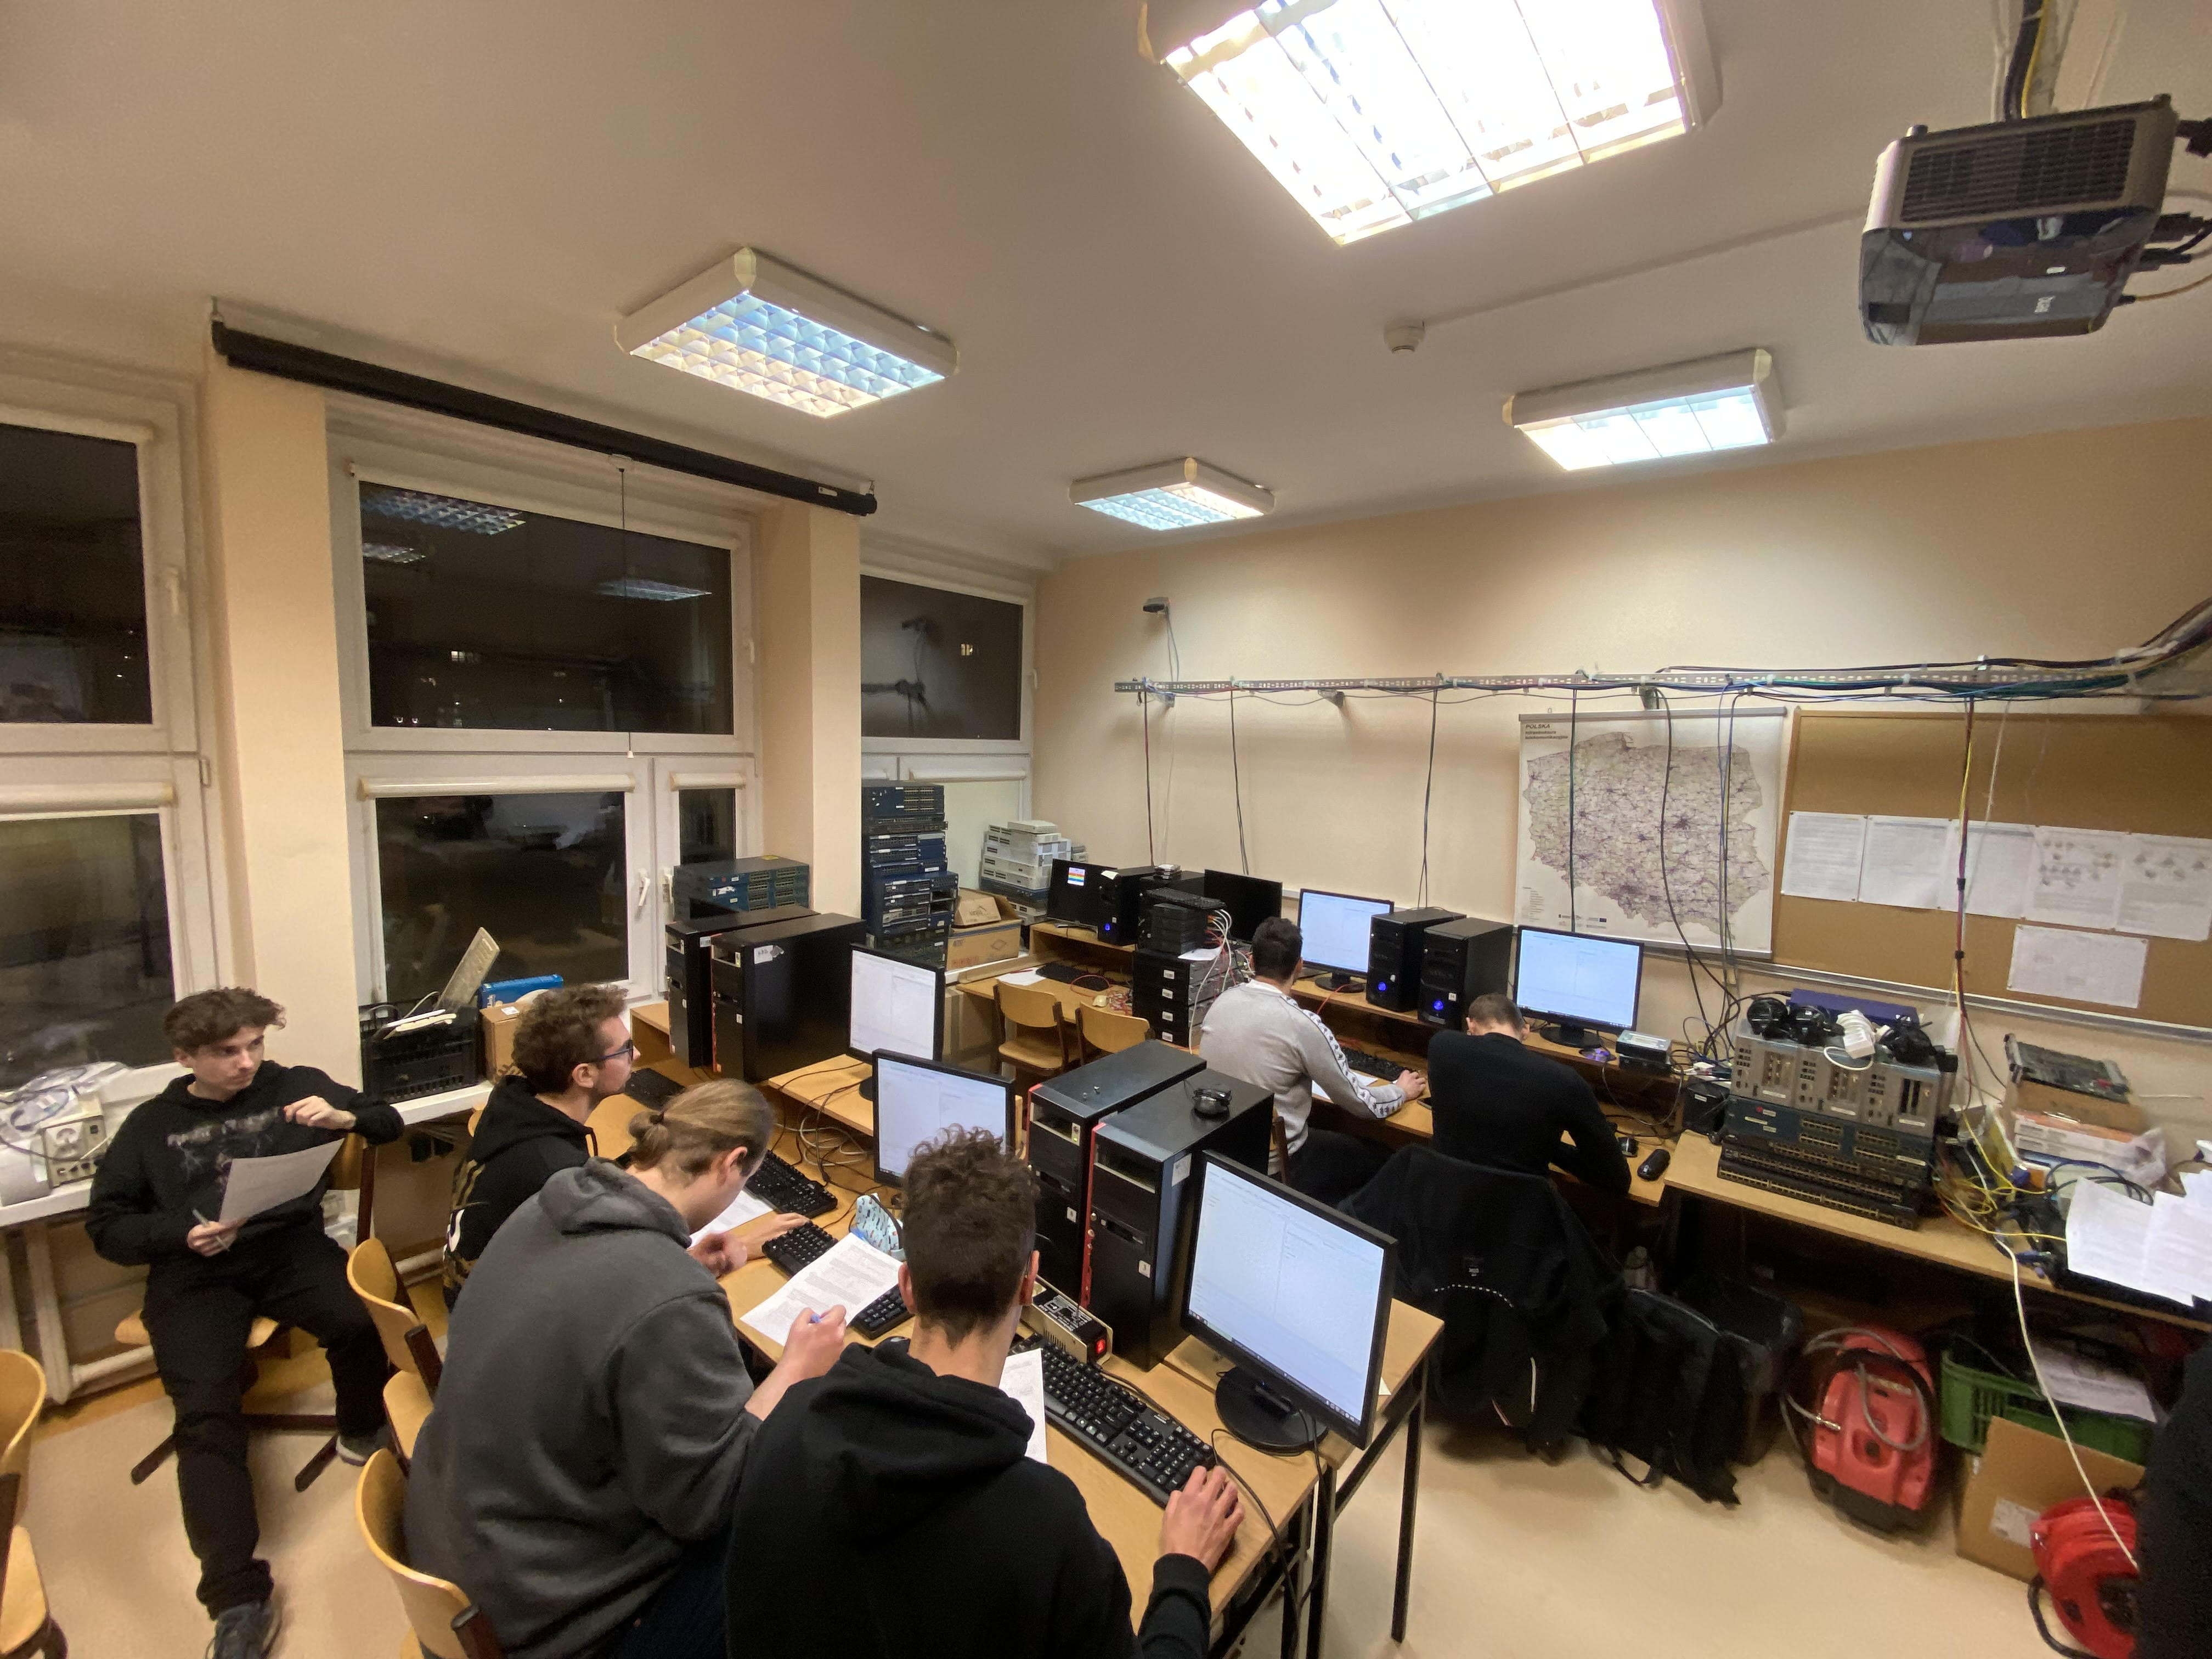
\includegraphics[width=\textwidth]{zajecia_lab.jpg}
    \caption{Zajęcia laboratoryjne przeprowadzone 6 grudnia 2023 r.}
    \label{fig:zajecia_lab_zdjecie}
\end{figure}

Za całość laboratorium studenci mogli uzyskać maksymalnie 4 punkty, w tym: 2 punkty za wejściówkę oraz 2 punkty za zadania laboratoryjne. Prace zostały ocenione w ciągu dwóch dni.

\subsubsection{Problemy}
Podczas zajęć również napotkano pewne problemy:
\begin{itemize}
    \item Przed zajęciami należało wgrać najnowszą wersję symulatora, okazało się to na tyle czasochłonne, że zajęcia rozpoczęły się z opóźnieniem około 15 minut,
    \item Studenci znaleźli błąd w symulacji PAM, który został naprawiony przed zajęciami z kolejną grupą.
\end{itemize}

\subsubsection{Wnioski}
Zarówno instrukcja, jak i symulator okazały się zrozumiałe dla studentów mających z nimi styczność pierwszy raz. System operacyjny nie miał żadnego wpływu na pracę studentów, ponieważ całość odbywała się w oknie symulatora. Zadania były wykonywane sprawnie, a poza pytaniami uczestnicy byli w stanie prowadzić dyskusję z prowadzącymi na temat rozwiązań i treści zadań.

Studenci otrzymali bardzo dobre oceny za wykonaną pracę, uśredniając: 95.9\% za całość, 97.2\% za wejściówkę oraz 94.6\% za część laboratoryjną. Spośród zadań na wejściówce jedyne problemy sprawiały zadania 5 i 6, a z zadań laboratoryjnych nieznacznie trudniejsze okazały się zadania związane z kodowaniem Reeda-Solomona.
